% \date{May 14, 2024}
% \author{Deralive / Shichien}
% \title{华东师范大学软件学院实验报告模板}
% 注意事项:编译两次,以确保目录、页码完整显示
% 模板文件:https://github.com/Shichien/ECNU-LateX-Template

\def\allfiles{}

\documentclass[14pt,a4paper,UTF8,twoside]{article}

\usepackage{amsmath}
\usepackage{graphicx}
\usepackage{longtable}
\usepackage{geometry} 
\usepackage{ctex}
\usepackage{booktabs} % 表格库
\usepackage{titlesec} % 标题库
\usepackage{fancyhdr} % 页眉页脚库
\usepackage{lastpage} % 页码数库
\usepackage{listings} % 代码块包
\usepackage{xcolor}
\usepackage[hidelinks]{hyperref}
\usepackage{tikz}
\usepackage{tikz-qtree}
\usepackage{fontspec} % 允许设置字体
\usepackage{unicode-math} % 允许数学公式使用特定字体
\usepackage{mwe}
\usepackage{zhlipsum} % 中文乱数文本
\usepackage{amsmath}
\usepackage{xcolor}
\usepackage{float} % 浮动体环境
\usepackage{subcaption} % 子图包
\usepackage{biblatex}
\usepackage{forest}
\addbibresource{references.bib} % 指定你的.bib文件名称

\definecolor{mygreen}{rgb}{0,0.6,0}
\definecolor{mygray}{rgb}{0.5,0.5,0.5}
\definecolor{mymauve}{rgb}{0.58,0,0.82}

\date{} % 留空,以让编译时去除日期

%———————————————注意事项—————————————————%

% 1、如果编译显示失败,但没有错误信息,就是 filename.pdf 正在被占用
% 2、在文件夹中的终端使用 Windows > xelatex filename.tex 也可编译

%—————————————华东师范大学———————————————%

% 论文制作时须加页眉,页眉从中文摘要开始至论文末
% 偶数页码内容为:华东师范大学硕士学位论文,奇数页码内容为学位论文题目

%————————定义 \section 的标题样式————————%

% 注意:\chapter 等命令,内部使用的是 \thispagestyle{plain} 的排版格式
% 若需要自己加上页眉,实际是在用 \thispagestyle{fancy} 的排版格式
% 加上下面这一段指令,就能够让 \section 也使用 fancy 的排版格式
% 本质就是让目录、第一页也能够显示页眉、页脚

\fancypagestyle{plain}{
  \pagestyle{fancy}
}

\title{华东师范大学软件学院课程项目报告} % 模板
\titleformat{\section}
    {\normalfont\bfseries\Large} % 字体大小、字体系列(\bfseries 为加粗)
    {\thesection}{1em}{}

% 设置章节的中文格式
\renewcommand\thesection{\chinese{section} \hspace{0pt}}
\renewcommand\thesubsection{\arabic{subsection} \hspace{0pt}}
% \renewcommand\thesubsubsection{\alph{subsubsection} \hspace{0pt}} % 字母编号
% \hspace{0pt} 是为了确保在章节编号和章节题目之间不要有空格,使得排版更为美观
    
%—————————————页面基础设置———————————————%

\geometry{left=10mm, right=10mm, top=20mm, bottom=20mm}

%————————————设置页眉、页脚——————————————%

\pagestyle{fancy} % 设置 plain style 的属性

% 设置页眉
% 使用 \footnotesize 确保章节名和标题名不会重合(缩小字体)

\fancyhead[RE]{\footnotesize \leftmark} % Right Even 偶数页右侧显示章名 \leftmark 最高级别章名
\fancyhead[LO]{\footnotesize \rightmark} % Left Odd 奇数页左侧显示节名 \rightmark 第二级别节名
\fancyhead[C]{华东师范大学软件学院课程项目报告} % Center 居中显示
\fancyhead[LE,RO]{~\thepage~} % 在偶数页的左侧,奇数页的右侧显示页码
\renewcommand{\headrulewidth}{1.2pt} % 页眉与正文之间的水平线粗细

% 设置页脚:在每页的右下脚以斜体显示书名

\fancyfoot[RO,RE]{\it Lab Report By \LaTeX} % 使用意大利斜体显示
\renewcommand{\footrulewidth}{0.5pt} % 页脚水平线宽度

% 设置页码:在底部居中显示页码

\pagestyle{fancy}
\fancyfoot[C]{\kaishu 第 \thepage 页 \ 共 \pageref{LastPage} 页} % LastPage 需要二次编译以获取总页数

%——————————————代码块设置———————————————%

\lstset {
    backgroundcolor=\color{white},   % choose the background color; you must add \usepackage{color} or \usepackage{xcolor}
    basicstyle=\footnotesize,        % the size of the fonts that are used for the code
    breakatwhitespace=false,         % sets if automatic breaks should only happen at whitespace
    breaklines=true,                 % sets automatic line breaking
    captionpos=bl,                   % sets the caption-position to bottom
    commentstyle=\color{mygreen},    % comment style
    deletekeywords={...},            % if you want to delete keywords from the given language
    escapeinside={\%*}{*},           % if you want to add LaTeX within your code
    extendedchars=true,              % lets you use non-ASCII characters; for 8-bits encodings only, does not work with UTF-8
    frame=single,                    % adds a frame around the code
    keepspaces=true,                 % keeps spaces in text, useful for keeping indentation of code (possibly needs columns=flexible)
    keywordstyle=\color{blue},       % keyword style
    % language=Python,               % the language of the code
    morekeywords={*,...},            % if you want to add more keywords to the set
    numbers=left,                    % where to put the line-numbers; possible values are (none, left, right)
    numbersep=5pt,                   % how far the line-numbers are from the code
    numberstyle=\tiny\color{mygray}, % the style that is used for the line-numbers
    rulecolor=\color{black},         % if not set, the frame-color may be changed on line-breaks within not-black text (e.g. comments (green here))
    showspaces=false,                % show spaces everywhere adding particular underscores; it overrides 'showstringspaces'
    showstringspaces=false,          % underline spaces within strings only
    showtabs=false,                  % show tabs within strings adding particular underscores
    stepnumber=1,                    % the step between two line-numbers. If it's 1, each line will be numbered
    stringstyle=\color{orange},      % string literal style
    tabsize=2,                       % sets default tabsize to 2 spaces
    % title=Python Code              % show the filename of files included with \lstinputlisting; also try caption instead of title
}

% 注释掉的部分用于后续插入代码,参数可调整,格式如下:

% 1、直接插入
% \begin{lstlisting}[language = ? , title = { ? } ]
%       Your code here.
% \end{lstlisting}

% 2、文件插入
% \lstinputlisting[language = C , title = ?.c] {filename.c}

%———————————————字体设置————————————————%

% \setCJKmainfont{SimSun} % 设置正文罗马族的 CJK 字体
% \renewcommand{\normalsize}{\fontsize{12pt}{15pt}\selectfont} % 设置正文字号
\linespread{1.2}

%———————————————超链接设置——————————————%

\hypersetup{
    pdfstartview=FitH, % 设置PDF文档打开时的初始视图为页面宽度适应窗口宽度(即页面水平适应)
    CJKbookmarks=true, % 用对CJK(中文、日文、韩文)字符的书签支持,确保这些字符在书签中正确显示
    bookmarksnumbered=true, % 书签带有章节编号。这对有章节编号的文档很有用
    bookmarksopen=true, % 文档打开时,书签树是展开的,方便查看所有书签
    colorlinks, % 启用彩色链接。这样,链接在PDF中会显示为彩色,而不是默认的方框
    pdfborder=001, % 设置PDF文档中链接的边框样式。001 表示链接周围没有边框,仅在单击时显示一个矩形
    linkcolor=blue, % 设置文档内部链接(如目录中的章节链接)的颜色为蓝色
    anchorcolor=blue, % 设置锚点链接(即目标在同一文档内的链接)的颜色为蓝色
    citecolor=blue, % 设置引用(如文献引用)的颜色为蓝色
}

%——————————————导言区结束,进入正文部分———————————————%

%——————————————————————————————————————%

\begin{document}

\maketitle

\begin{center} % \extracolsep{\fill} 拉伸到页面最大宽度前,保证居中显示

    \begin{tabular*}{\textwidth}{@{\extracolsep{\fill}} l  l  l }
        \hline
        课程名称:Linux 应用编程 & 成绩:\\
        姓名:张梓卫 & 学号:10235101526 \\
        指导老师:徐刚 & 日期:2024/10/10 \\
        作业名称:Linux 文件系统 & 班级:软工3班\\
        \hline
    \end{tabular*}

\end{center}

\tableofcontents % 目录也需要二次编译

%————————————————————————————————————————————————————————————

\section{课后练习 1}

\subsection{创建目录文件夹}

使用 mkdir 命令创建目录文件夹,再使用cd命令进入,如:

\begin{lstlisting}[language = bash, title = {创建目录文件夹}]
  mkdir 10235101526_Linux2024
  ls
  cd 10235101526_Linux2024
\end{lstlisting}

\begin{figure}[H]
\centering
    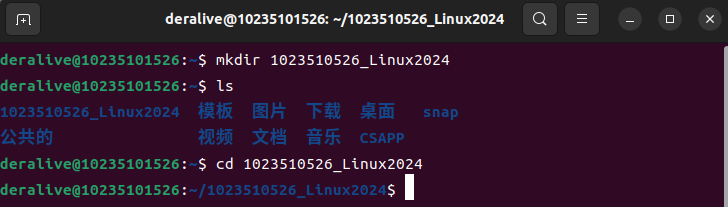
\includegraphics[width=0.8\textwidth]{lec2/mkdir.png}
    \caption{创建目录文件夹}
    \label{fig:1}
\end{figure}

\subsection{向目标文件foo中写入内容}
使用 echo 命令向目标文件foo中写入内容,如:

\begin{lstlisting}[language = bash, title = {向目标文件foo中写入内容}]
  echo -e "10235101526\n" > foo
\end{lstlisting}

其中,-e参数用以启用转义字符的解释功能。

\subsection{向目标文件中追加内容}
使用 cat 命令向目标文件中追加内容,如:

\begin{lstlisting}[language = bash, title = {向目标文件中追加内容}]
  cat /etc/passwd >> foo
\end{lstlisting}

\begin{figure}[H]
  \centering
    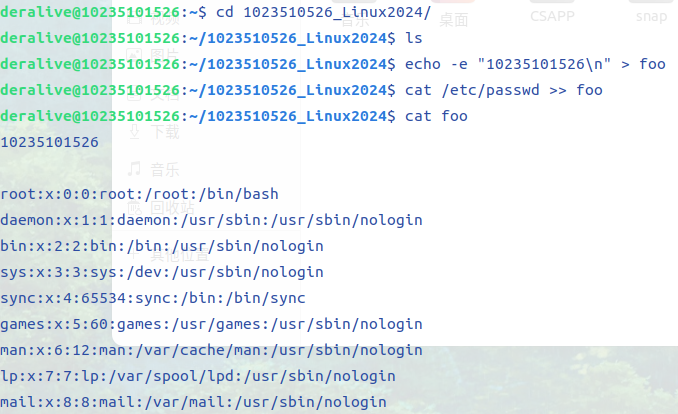
\includegraphics[width=0.6\textwidth]{lec2/cat.png}
    \caption{向目标文件中追加内容}
    \label{fig:2}
\end{figure}

\subsection{对目标文件进行权限修改}

通过课上讲授的内容,对chmod命令进行使用,其中八进制权限如下所示。

对于当前用户,是前三位,中三位是所有者,后三位是其他用户。

\begin{figure}[H]
  \centering
  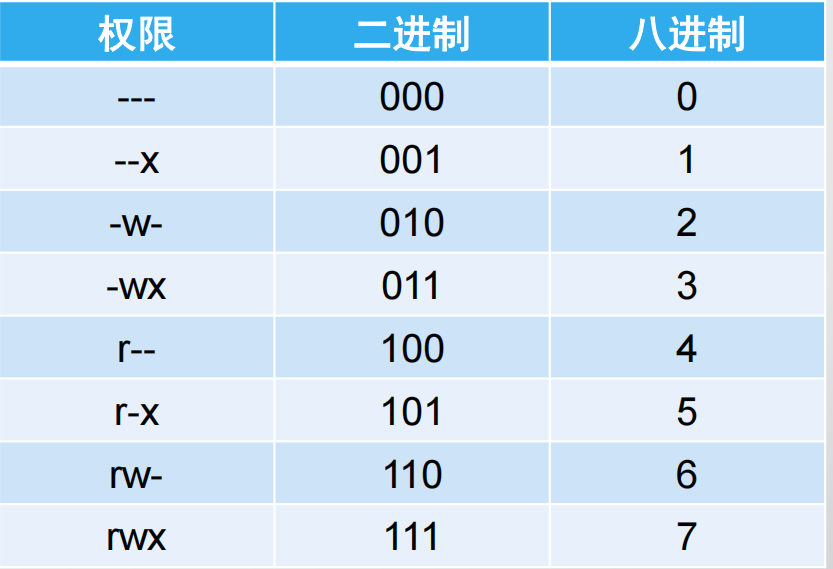
\includegraphics[width=0.3\textwidth]{lec2/privilege.png}
  \caption{对目标文件进行权限修改}
  \label{fig:3}
\end{figure}

根据上述分析,我们应该使用以下命令:

\begin{lstlisting}[language = bash, title = {对目标文件进行权限修改}]
  chmod 400 foo
\end{lstlisting}

\subsection{修改文件的修改时间}

使用touch命令即可。

\begin{lstlisting}[language = bash, title = {修改文件的修改时间}]
  touch -t 202409200000 foo
\end{lstlisting}

\subsection{创建seeme文件}

\begin{lstlisting}[language = bash, title = {创建seeme文件}]
  mkdir secret
  echo "Contents" > secret/seeme
  chmod 600 secret/seeme
\end{lstlisting}

执行情况如下所示:

\begin{figure}[H]
  \centering
  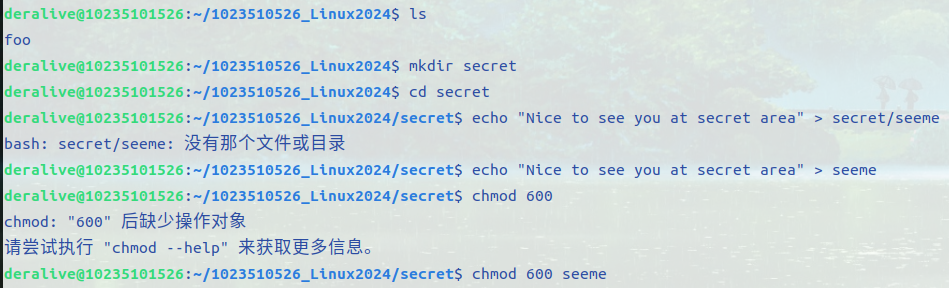
\includegraphics[width=0.5\textwidth]{lec2/chmod.png}
  \caption{创建seeme文件}
  \label{fig:4}
\end{figure}

\subsection{创建一个新用户}

\begin{lstlisting} [language = bash, title = {创建一个新用户}]
  sudo adduser deraliveson
  su deraliveson
  cat 10235101526_Linux2024cat/secret/seeme
\end{lstlisting}

切换用户后,查看文件内容失败。

\begin{figure} [H]
  \centering
  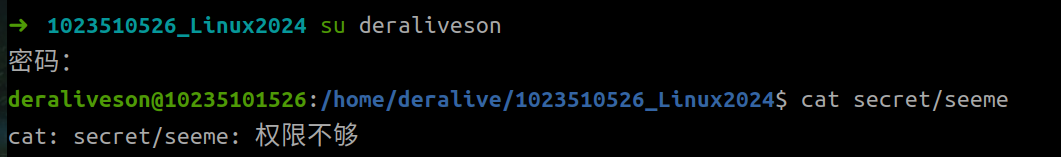
\includegraphics[width=0.5\textwidth]{lec2/deraliveson.png}
  \caption{查看内容失败}
  \label{fig:5}
\end{figure}

\section{课后练习 2}
\subsection{修改目标文件,创建硬链接}

注意:这里题目要求在学号的目录之下创建硬链接和符号链接

\begin{lstlisting} [language = bash, title = {修改目标文件,创建硬链接}]
  ln secret/seeme see-hlink
  echo "change at see" > secret/seeme
\end{lstlisting}

\begin{lstlisting} [language = bash, title = {查看硬链接}]
  cat secret/seeme
  cat see-hlink
\end{lstlisting}

硬链接(hard link)是Linux和UNIX文件系统中的一种文件链接方式,它允许多个文件名指向同一个文件数据。每个硬链接都是该文件的一个等效副本,指向相同的数据块,因此无论哪个硬链接被访问或修改,实际存储的数据都保持一致。

硬链接 (ln):指向文件内容,即使源文件被删除,硬链接依然可以访问文件内容。

符号链接 (ln -s):指向文件的路径,如果源文件被删除,符号链接会变为无效链接。

\begin{figure} [H]
  \centering
  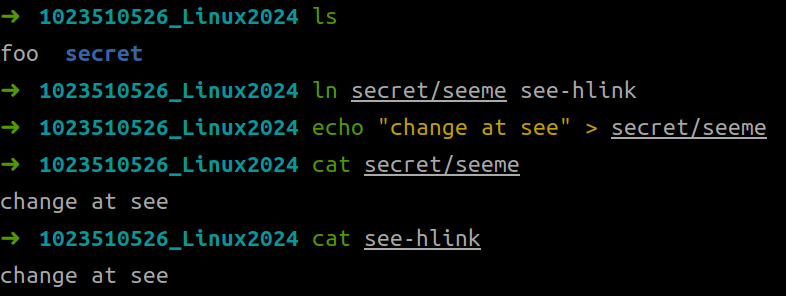
\includegraphics[width=0.5\textwidth]{lec2/hlink.png}
  \caption{创建硬链接}
  \label{fig:6}
\end{figure}

\subsection{Debug: 无法进入目录}

发现创建的文件夹存在权限问题,所以切换了deraliveson用户之后,是无法看到deralive的目录的,于是切换回去修改权限。

该过程如下所示:

\begin{figure}[H]
  \centering
  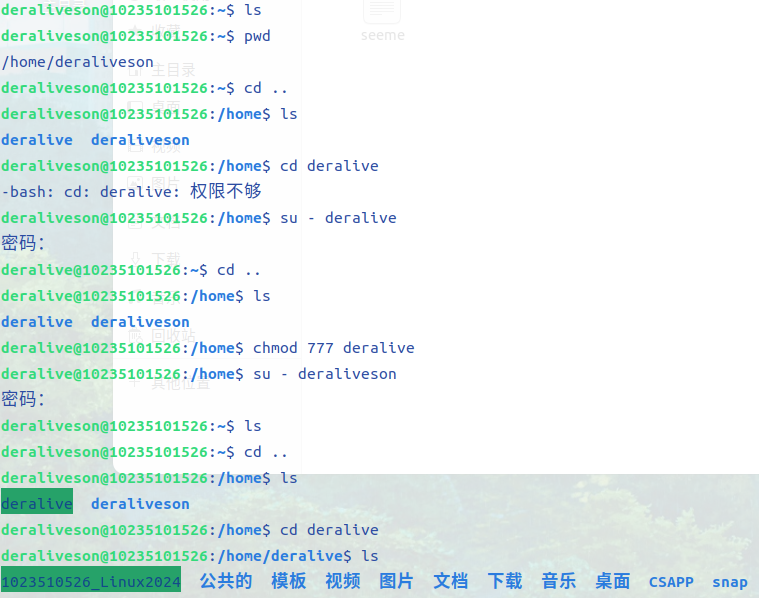
\includegraphics[width=0.5\textwidth]{lec2/visionable.png}
  \caption{Debug: 无法进入目录}
  \label{fig:7}
\end{figure}

使用的命令如下所示:

\begin{lstlisting} [language = bash, title = {Debug: 无法进入目录}]
  cd ..
  sudo chmod 777 deralive
  sudo chmod 777 deralive/10235101526_Linux2024
  sudo chmod 777 deralive/10235101526_Linux2024/secret
  su - deraliveson
  cd 10235101526_Linux2024/secret
\end{lstlisting}

\subsection{使用另一个用户查看文件内容}

\begin{lstlisting}
  su deraliveson
  cd ..
  cat deralive/10235101526_Linux2024/secret/seeme
  cat deralive/10235101526_Linux2024/secret/see-hlink
\end{lstlisting}

\textbf{注意:此命令后来装了autojump之后,可以更简单地操作}

即:

\begin{lstlisting} [language = bash, title = {使用另一个用户查看文件内容}]
  su deraliveson
  cat secret/seeme
  cat see-hlink
\end{lstlisting}

提示权限不足:

\begin{figure} [H]
  \centering
  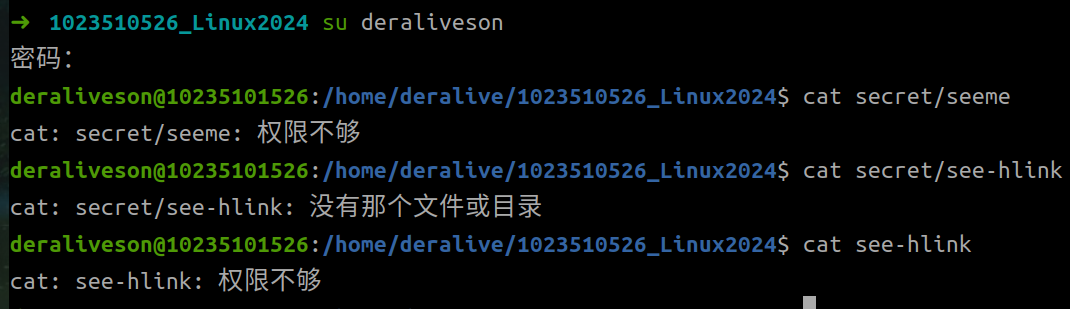
\includegraphics[width=0.5\textwidth]{lec2/cantcat.png}
  \caption{提示权限不足}
  \label{fig:8}
\end{figure}

\subsection{创建符号链接}
\begin{lstlisting} [language = bash, title = {创建符号链接}]
  ln -s secret/seeme see-slink
  echo "change at see-slink" > secret/seeme
\end{lstlisting}

用另一个账户同样去查看seeme和see-slink的内容,仍然提示无权限。

\begin{lstlisting} [language = bash, title = {提示权限不足}]
  su deraliveson
  cat secret/seeme
  cat see-slink
\end{lstlisting}

\begin{figure}[H]
  \centering
  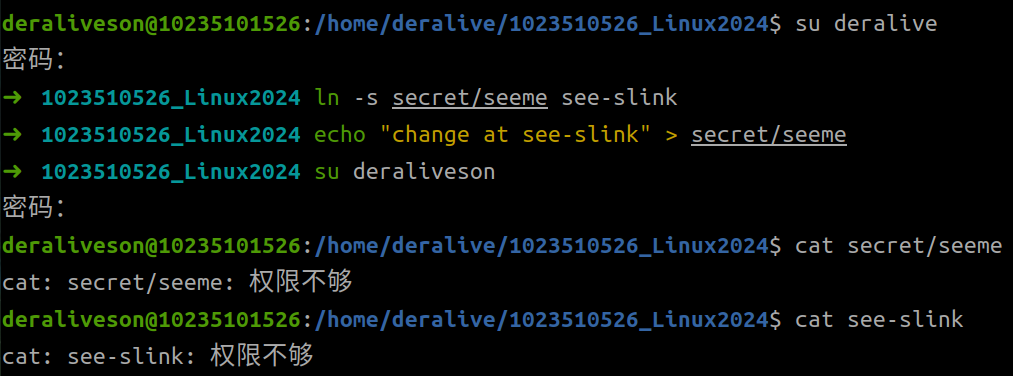
\includegraphics[width=0.5\textwidth]{lec2/alsocant.png}
  \caption{提示权限不足}
  \label{fig:9}
\end{figure}

\subsection{只有硬链接能仍然访问内容}

\begin{lstlisting} [language = bash, title = {只有硬链接能仍然访问内容}]
  cd secret
  rm seeme
  cd ..
  cat see-slink
  cat see-hlink
\end{lstlisting}

\begin{figure} [H]
  \centering
  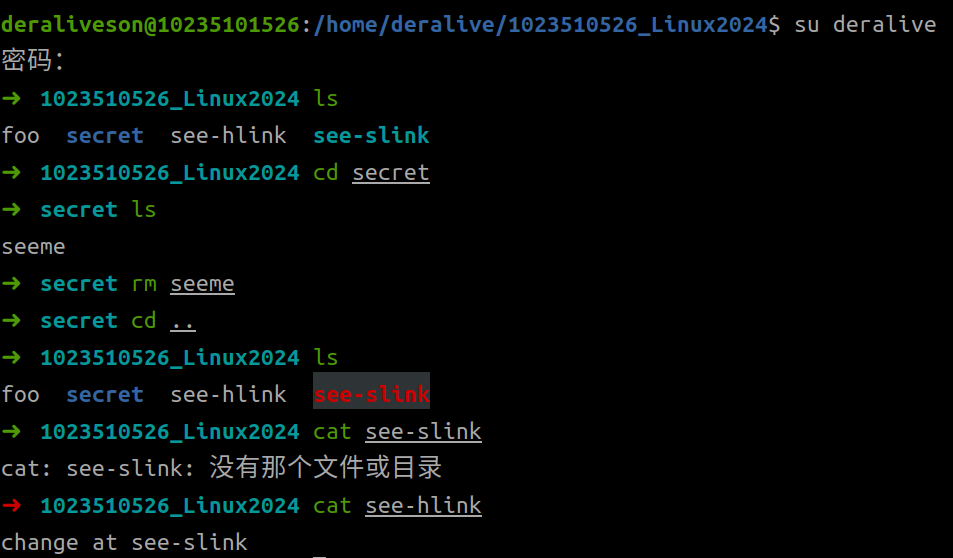
\includegraphics[width=0.5\textwidth]{lec2/final.png}
  \caption{只有硬链接能仍然访问内容}
  \label{fig:10}
\end{figure}

\section{目录打包}

\subsection{给文件打包}

\begin{lstlisting} [language = bash, title = {给文件打包}]
  tar -czvf 10235101526_Linux2024.tar.gz 10235101526_Linux2024
  cp 10235101526_Linux2024.tar.gz 10235101526_Linux2024/
\end{lstlisting}

通过这两条指令实现打包和复制压缩包到原目录当中。

\begin{figure} [H]
  \centering
  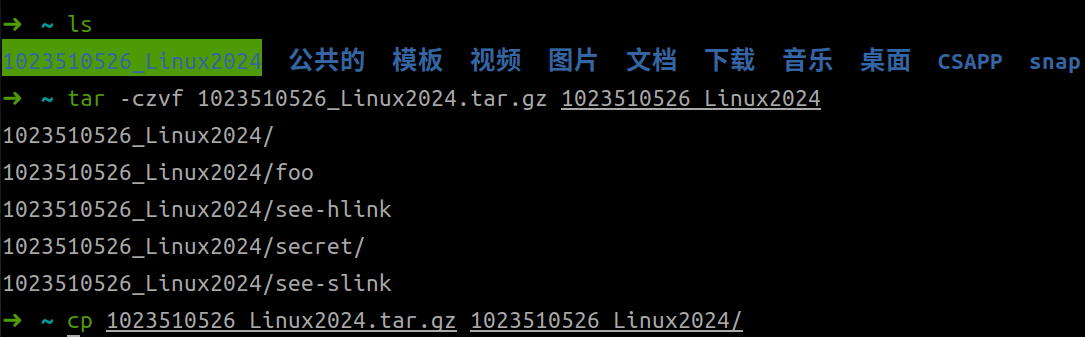
\includegraphics[width=0.5\textwidth]{lec2/tar.png}
  \caption{给文件打包}
  \label{fig:11}
\end{figure}

\section{捣鼓 Linux 美化}

使用 Oh My Zsh 进行美化,安装代码补全工具,使用autojump进行目录跳转。

参考资料:

\begin{itemize}
  \item \href{https://github.com/wting/autojump}{\underline{https://github.com/wting/autojump}}
  \item \href{https://www.jianshu.com/p/35157cef7a43}{\underline{https://www.jianshu.com/p/35157cef7a43}}
\end{itemize}

\section{其余学习到的内容}

\subsection{VMware 建立代理}
注意 VMnet1 与 VMnet8 ,若出现了169.254.X.X,这是Windows操作系统在DHCP信息租用失败时自动给客户机分配的IP地址。69.254.X.X的分配可能会令客户机与所处局域网网关(Modem,路由器,或提供共享上网的主机)位于不同的网段中,而无法与网关通信,而导致无法接入Internet的情况。

参考:\href{https://www.cnblogs.com/daxian1607212422/articles/17869141.html}{\underline{https://www.cnblogs.com/daxian1607212422/articles/17869141.html}}

\subsection{root 用户}
用su - root可以切换到root用户,输入的是root用户的密码,但是Ubuntu默认root用户是没有密码的,你得为root用户设置一个密码才能用root用户登录:
sudo passwd root

\subsection{更改字体大小}
使用 Ctrl + Shift + + 变大
使用 Ctrl + - 变小

\newpage{}

\section{附录}

\end{document}